\documentclass[11pt]{article} 
\usepackage{graphicx}
\usepackage{amsmath,amssymb}
\usepackage{tikz}
\usepackage{textcomp}
\usepackage{braket}
\usepackage[shortlabels]{enumitem}

\newcommand{\doctitle}{ }
\makeatletter
\renewcommand{\ps@headings}{%
\renewcommand{\@evenhead}{\parbox{\textwidth}{\hrulefill
\fbox{\sffamily Astro Cosmology}\hrulefill } }%
\renewcommand{\@oddhead}{\parbox{\textwidth}{\hrulefill 
\fbox{\sffamily Astro Cosmology}\hrulefill}}}
\makeatother


\linespread{.9}
\hoffset=-0in    \voffset=-.5in
\oddsidemargin=0in   \evensidemargin=0in
\topmargin=-.25in
\textwidth=6.5in   \textheight=9.5in
\columnseprule=.3pt  
\setlength{\parskip}{1em}



\usepackage{multirow}
\usepackage{multicol} 
\usepackage{braket}

\newcommand{\mytitle}[1]{{
\begin{centering}
{\Large \sffamily AstroCosmology}\\
\bigskip\bigskip{\Large \sffamily \bfseries{#1}}\\
\bigskip\bigskip\end{centering}
}}

\newcommand{\mytitlecompact}[1]{{

\hfill
{\Large \sffamily \bfseries{#1}}
\hfill
%\bigskip
}}

\newcommand{\mysection}[1]{{
\smallskip
\noindent
{\large \sffamily \bfseries{#1}}
}}


\newcommand{\mysubsection}[1]{{
\smallskip
{\sffamily \bfseries{#1}}
}}

\pagestyle{empty}
\pagestyle{headings}

\def\C{{\mathbb{C}}}
\def\R{{\mathbb{R}}}
\def\Q{{\mathbb{Q}}}
\def\Z{{\mathbb{Z}}}
\def\N{{\mathbb{N}}}
\def\cA{{\mathcal{A}}}
\def\cC{{\mathcal{C}}}
\newcommand{\expectation}[1]{\langle #1\rangle}
%\def\bra{\langle}
%\def\ket{\rangle}

\begin{document}
%\newcommand⟨\expectation⟩[1][]{$\langle$ #1 $\rangle$}
\begin{abstract}
    These are notes on physics I learned throughout my junior year outside of normal classes. 
\end{abstract}
\mytitlecompact{Notes on Astroparticle Physics and Cosmology}
\part{Particles}
\section{Fermi's Golden Rule}
\textbf{Fermi's Golden Rule} is used for calculating transition rates between particles. 
Assume there's a time-independent perterbation to the system, and thus to the Schrodinger equation
\begin{equation}
    i\frac{d \psi}{d t} = \left[H + H'\right]\psi
\end{equation}

Still expand $\psi = c_k \ket{k}e^{-iE_k t}$ in terms of (time dependent) energy eigenfunction will give us 
\begin{equation}
    i\sum_k \left[ \frac{d c_k}{dt}\ket{k}e^{-iE_k t}- i E_k c_k \ket{k}e^{-iE_kt}\right] =
    \sum_k c_k H \ket{k}e^{-iE_kt} + \sum_k c_k H' \ket{k}e^{-iE_kt}
\end{equation}
Use property of the imaginary numbers and the fact that we are operating under eigenstates, we can cancel the middle terms to get 
\begin{equation}
    i\sum_k \frac{d c_k}{dt}\ket{k}e^{-iE_k t} = \sum_k c_k H' \ket{k}e^{-iE_kt} \label{fermi golden rule 1st}
\end{equation}

If we do a dot product with $\bra{f}$, and assume only $c_i\approx 1$, others $c_k\approx 0$,
we would get 
\begin{equation}
    i \frac{d c_f}{dt} e^{-i E_f t} = \braket{f|H'|i}e^{-iE_i t}
\end{equation}
or 
\begin{equation}
    \frac{d c_f}{dt}  = -i \braket{f|H'|i}e^{-i(E_i- E_f)t}
\end{equation}
For simplicity, we just call $\braket{f|H'|i}:= T_{fi}$

The whole coefficient is $\int_0^T -i \braket{f|H'|i}e^{-i(E_i- E_f)t} dt$,
and the probability is just 
\[P_{fi} = |T_{fi}|^2 \int_0^T\int_0^T e^{-i(E_i- E_f)t} e^{i(E_i- E_f)t'} dt dt'\]
Note this is essentially $c_k c_k^*$, and we can relabel the dummy variable in integration so 
it won't change as the other changes. 

We define the transition rate as the the probability to transit within sometime, so it 
is 
\begin{equation}
    d\Gamma_{fi} = P_{fi}/T
\end{equation}
Moreover, we can simpify this a bit with $\int_\infty^\infty e^{i(k-k_0)} = 2\pi \delta(k-k_0)$,
\begin{equation}
    d\Gamma_{fi} = 2\pi \frac{|T_{fi}|^2}{T} \lim_{T\to \infty}\int_{T/2}^{T/2}e^{-i(E_i- E_f)t}\delta(E_i-E_f) dt
\end{equation}
The dirac delta essentially specify that $E_i\approx E_f$. Another thing we can do is to assume multiple $E_f$ are possible going from $E_i$.
So there are $dn$ states in $E_f\to E_f+dE_f$. If $n$ is the total number of states, then $\frac{dn}{dE_f}$ symbolizes how many states where added going through $E_f\to E_f+dE_f$. So it is an 
appropriate value for density of states. 

So the above becomes 
\begin{equation}
    d\Gamma_{fi} = 2\pi \int_{E_f}^{E_f+dE_f} \frac{dn}{dE_f}\frac{|T_{fi}|^2}{T} \lim_{T\to \infty}\int_{T/2}^{T/2}e^{-i(E_i- E_f)t}\delta(E_i-E_f) dt dE_f
\end{equation}

When we evaluate the integral by plugging in $E_f = E_i$,
the above just becomes, with the integral over $T/2$ to $-T/2$ cancel with $T$ to give 1, use $dE_f$ to cancel with 
1, the change of $E_f$ to $E_f+ dE_f$ combines density of states and the dirac deltat to give $\frac{dn}{dE_f}|_{E_i}$ 
$\Gamma_{fi} = 2\pi |T_{fi}|^2 \frac{dn}{dE_f}|_{E_i}$

Upgrading a little bit, we can plug in $c_f = - i \braket{f|H'|i}\int_0^T e^{-i(E_i-E_f)t}dt$
This makes (\ref{fermi golden rule 1st}) then (after dot product with $\bra{f}$)
\begin{equation}
    \frac{d c_f}{dt} = -i \braket{f|H'|i}e^{i (E_f-E_i) t} + (-i)^2 \sum_{k\neq i}\braket{f|H'|k} e^{i(E_f-E_k)}\int^t_0(\braket{k|H'|i})e^{i(E_k-E_i)t}dt
\end{equation}
Notice we switched expression for coefficient from $f$ to $k$.
This, after doing explicity integration assuming time-independent perturbation, we have, to \textbf{second order},
\begin{align}
    \frac{d c_f}{dt} &= -i \braket{f|H'|i}e^{i (E_f-E_i) t} + (-i)^2 \sum_{k\neq i}\braket{f|H'|k} e^{i(E_f-E_k)} \frac{\braket{k|H'|i}e^{i(E_k-E_i)t}}{i(E_k-E_i)}\\
    &= -i \braket{f|H'|i}e^{i (E_f-E_i) t} + (-i) \sum_{k\neq i}\braket{f|H'|k} e^{i(E_f-E_i)} \frac{\braket{k|H'|i}}{(E_k-E_i)}\\
\end{align}

Extract the common exponential factor and (-i), we get $T_{fi} = (-i) (\braket{f|H'|i}+ \sum_{k\neq i}\braket{f|H'|k}\frac{\braket{k|H'|i}}{(E_k-E_i)})$
\part{Cosmology}
\section{Baryon Acoustic Oscillations (BAO) \cite{BassetBAO}}
One of my most intersted topics in cosmology! 
BAO started off from coupling between photon and baryons with compton scattering. Because everything was hot, there were actually photon-baryon plasma
 and it oscillates due to interplay between gravitational potential and radiaition pressure. 
According to these canonical plot 
by Eisenstein, a purterbation would propage outwards as a sounds wave , and after decoupling photons
fly away, and baryons are left at around 150 Mpc position. At the bottom pictures, baryon and dark matter tend to drag the other toward themselves. The upshots is an overdensity of baryons and dark matter at the center and spherical halo of baryons on the outskirt.
You can solve for momentum conservation by expanding using mean free path of photons in fourier space, with gravity as source of perturbation. 
As the photon decouples, it is possible to characterize growth of amplitude of different modes.  

Higher order processes are generally on the scale of less than 150 Mpc, so it barely affects measurements of BAO. Larger systematic source of error (make the circle smaller or larger) are found to be canceling using technqiues including \textbf{Zel' dovich technique}. 
This makes BAO robust measurement of distance. 

Zel' dovich approxiamtion is an intuitive approxiamtion technique that succesfully predicts filament, clusters, voids, and sheets of the universe. 

\begin{center}
    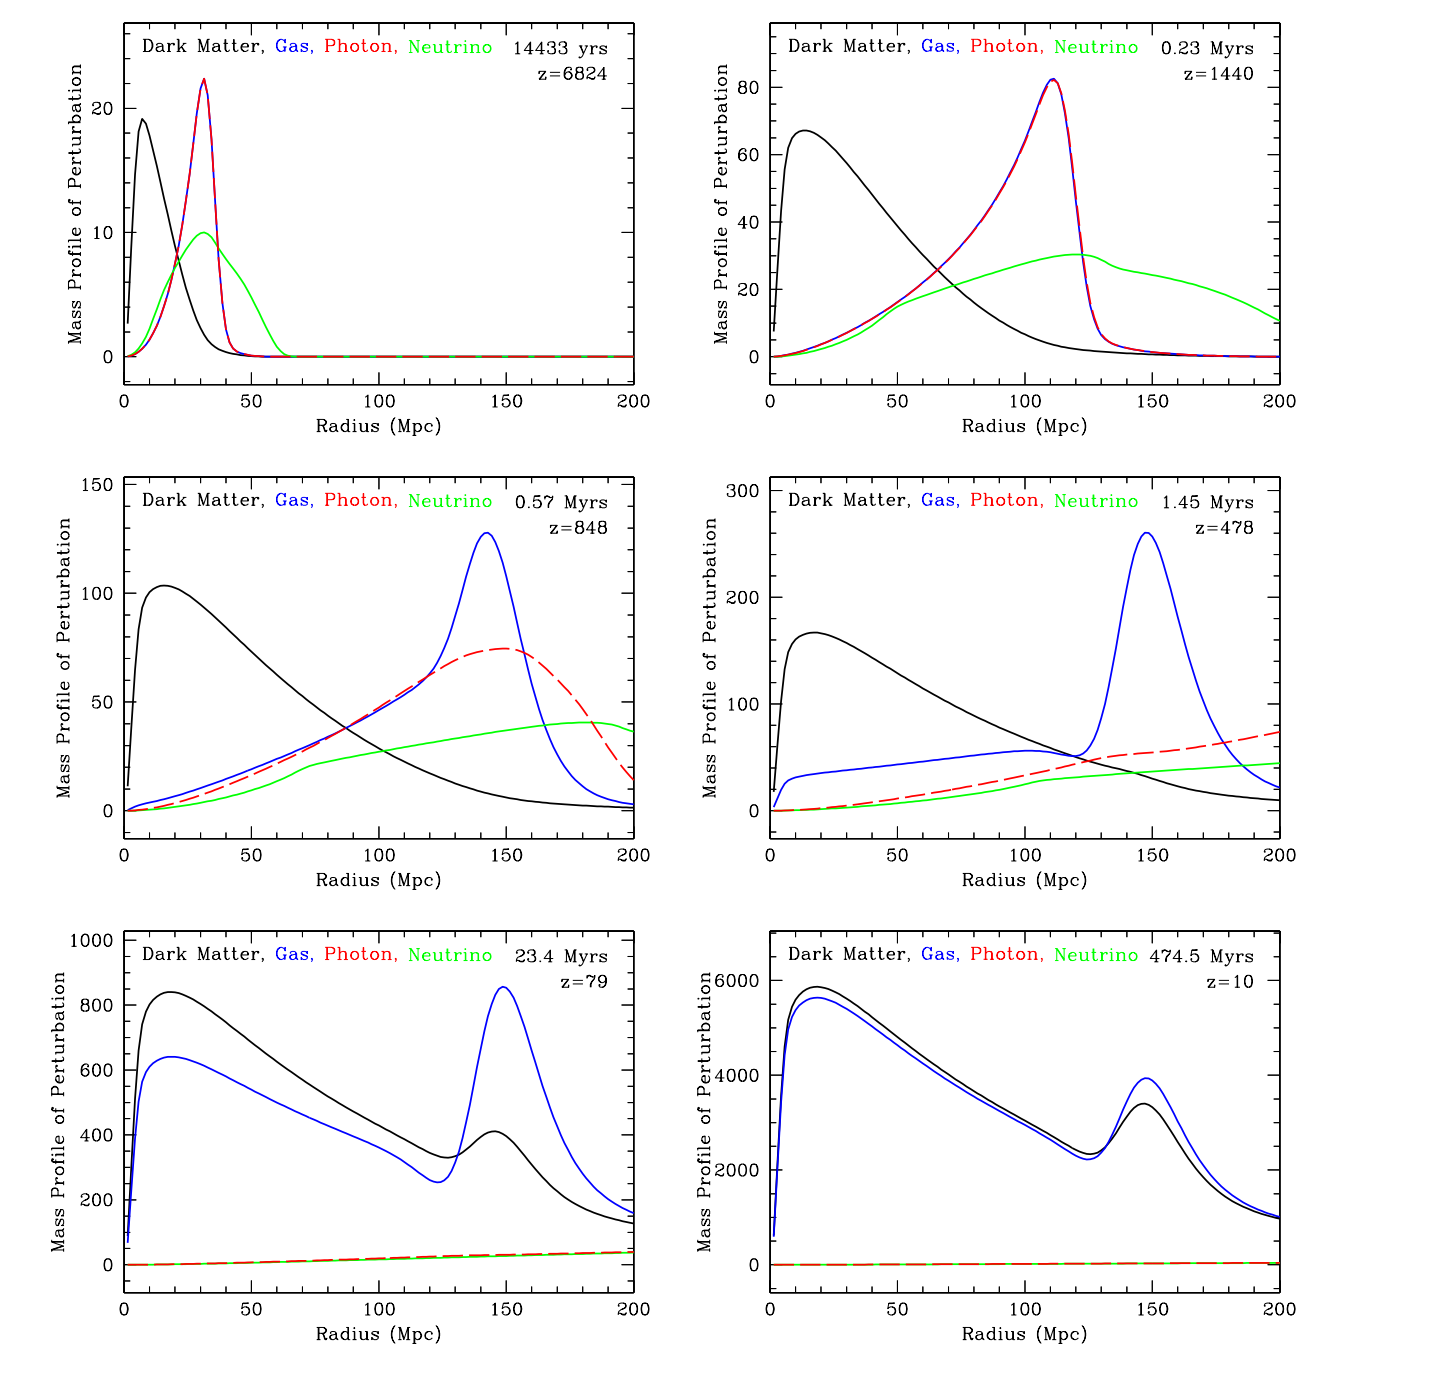
\includegraphics[scale=0.5]{BAO Evolution.png}
\end{center}

BAO serves as good \textbf{stabdard ruler} because it has known size at a certain wavelength and we know how its size changes with $z$. 
It is considered as a \textbf{statistical standard ruler (SSR)}. SSR assumes there's a favorite distance for stars to spread apart: an ideal situation would be you drop a galaxy, draw a circle with radius r, drop another galaxy on the circle, use the new galaxy as the center of a circle again\dots This is best seen in terms of two point correlation function.

In (this review article), we use the Friedmann equation to write dimensionless hubble constant using info on dark energy density and other cosmological constants.
With dark energy as a \textbf{barotropic fluid} (density only depends on pressure), and we can write equation of state of dark energy in terms of redshift dependence (w(z)). This can be contrained using distance measurements. 
Some distance measurements are determined with the comoving distance ($r$ in Ryden, $\chi$ in weinberg and others) and curvature. \textbf{Angular diameter distance} $d_A$ and \textbf{luminosity distance} $d_L$.

In review article, with the help of \textbf{Alcock-Paczynski test} (evaluation of the ratio of observed angular size to radial/redshift size, it uses the fact that circlular object becomes elliptical when viewed slanted), we get value of $d_A(z)$ and $H$
together. 

If the two point correlation function $\xi$ has and only has 1 peak, then its fourier transform will be a perfect $\sin$ wave. This is the power spectrum. By measuring both on BAO, much more information can be extracted and BAO can provide better constaints on cosmological parameters.

\section{First Stars}
Also one of the hottest topics in cosmology/astrophysics research. It offers info on the histroy of structure formation and the chemicals in early ages of universe. 

Most popular opinion is that primordial gas form in low-mass halos and then are cooled through molecular hydrogen cooling. Radiation can eitehr stop the formation process by dissociating molecular hydrogen or use X-ray to promote $\text{H}_2$ production. 

\subsection{Brief Summary Of \cite{naoki03a}}
With an $N-$body simulation with nine chemical species, electro, hydrogen (ionized or not), helium atom and gas, using the GADGET code, some cosmological parameter and cooling rate determined by other scholars, we advanced the time evolution. 
After simulation we then search for dark matter halos and look for promising gas clouds. We found that there's a critical line as a function of fraction of $\text{H}_2$ and tempterature $T$ that determines whether the clouds were able to cool or not. 
Function of this line can be theoretically calculated. 

Accounting for the size of the halo, we note the faster it accretes, the harder it is to cool, which came from the dynamical heating. Therefore we can find a critical growth rate of halos. Similar phenomenon occurs with too much mass. 
The initial angular momentum of gas may determine property of gas clouds. Especially, a fast spinning system may form a disk like structure. It turns out system with high \textbf{spin parameter} is pretty hard to find. The spin parameter does affect the shape of the gas
 coulds formed. 
We then fitted a spherical collapse model to the cooling of the gas clouds in our simulation, the agreement is great. 

Accounting for uniform backgroud radiation in the LW band and self-shielding, we found that radiation does prevents cooling significantly, and self-shielding is less affective with small (optically thin objects). 

In order to run bigger simulations, we intend to couple a N-body simulation with some semianaltic model. We accounted for radiation during the formation of stars and modeled gas formation pattern. We then use some simulation just with CDM particles and got agreeing results. 

\section{Line Intensity Mapping (LIM)\cite{KovetzStatusReport}}
\subsection*{Overview}
LIM is the next generation of detection method, that can probe larger areas faster, cheaper, and deeper into high redshifts, compared to normal galaxy surveys. This is because Galaxies must be bright enough in high $z$ regions for it to be detected by telescope; but LIM can deal with unresolved galaxies, as it takes the noise as part of its analysis as well. Because dilution of aggregated signal is less sever than dilution of signal from 1 galaxies as redshift increases.

LIM takes in spatial fluctions (large scale structre) in many unresolved galaxies, and the frequency dependence of these fluctation tells us ditribution of emission. The power spectrum contains information on the clustering and shot noise (modeled by Poisson process, came from discrete sampling of galaxies), redshift bias, and average intensity. The spectrum depends on DM fluctuation and other astrophysical processes. 

\subsection*{What LIM Does}
Neutrino dynamics is very different from CDM and Baryon matters, because they are traveling fast, leaving signatures on observables. Pairing galaxy survey with hydrodynamics simulation, one may contraint the mass of neutrino well enough. 

Of course, we also want to contrain the cosmological constants better. But notice, both astrophysical process and cosmological parameter affect emission lines. Therefore, we need to either pair LIM results with simulation, cross correlate different methods of observation, or use analytical methods (e.g. redshift space distortion, how stars are elongated towards us in redshift space) to get rid of density fluctuations caused by astrophysical phenomenon. 

By plotting predictions of Horndeski and quintessence models for gravity, we found that their deviation from Benchmark model differ at high redshft ($z>2$), and LIM can just probe into that. 
Other alternative theories LIM can probe include: heating of dark matter by annilation, collision between DM and baryon $\ldots$.  We need $z>20$ probe for these information to be extracted. 

Because current measurement into deep stars need the stars to be bright, there is a biased sampling in selecting targets for studying the first stars. Carbon-monoxide intensity mapping is the better method to delve into primodrial gas. This determines the star-forming-gas reservoir at high redshifts. 

\subsection*{How LIM Does It}
One can correlated LIM with overlapping galaxy surveys (not so hard to find one due to large area probed by LIM). This can be used to filter out contaimation due to say dusts and synchrotron radiation (foreground contamination). 

We also need to model astrophysical/cosmological process happens in LIM pictures. This helps us predict signal to noise ratio and interpret results of the surveys. 
We can empirically interpolate line luminosity and halo mass, and use halo model to compute say power spectrum. The other way is to run numerical simulations and apply known physics to the results (semi-analytic). 

\section{Cosmic Bell Test}
Using (high $z$) quasars to test quantum theory. 
\subsection*{Entanglement} 
1930s, QM community began to study Entanglement. A. Einstein, B. Podolsky, N. Rosen made paper that behavior of particle $B$ seems to be depend on particle $A$ \textbf{instantaneously}, even they are arbitrarily far. 
\begin{equation}
    \ket{\psi} = \frac{1}{\sqrt{2}}(\ket{u}_A\ket{v}_B + \ket{v}_A\ket{u}_B)
\end{equation}
This does not factorize, based on local realism. 

Bell test:
\begin{enumerate}
    \item dichotomic observables. $A(a), B(b) = \pm 1$. Say we have 2 SG devices. 
    \item $E(a,b) = \braket{A(a)B()b}$. Does the measure the same or opposite? 
    \item Vary question asks by 
    \item EPR predicts an upperbound for $S = E(a,b) + E(a',b) + E(a, b') - E(a',b')$ of 2
    \item But QM says $S_{max} = 2\sqrt{2}$. 
\end{enumerate}

Early results at LBL by John Clauser, 1972. $|S|>2$ by $5\sigma$. Recently, Jian-Wei Pan, $|S|>2$ by $4.1\sigma$. 

\subsection*{Loop holes}
\begin{enumerate}
    \item Locality Loophole: hidden communication between parties: information is transmitted during difference between measurements. Need spacelike spearated arrangement. 
    \item Detector Efficiency loophole $\to$ detector fails to respond. 
    \item \textbf{Freedom of choice loophole}. Whether properties of particle correlated to questions being asked. Whether the type of measurement is entirely independent and random. The assumption was choice of detector setting was correlated with particle property. 
    Only a small such correlation can reproduce what has been observed. 
\end{enumerate}

Some used volunteers to play games to generated randomness. 

\subsection*{Cosmic Bell Test}
Conformal times ($\tau = \int^{t0}_0 \frac{dt'}{a(t')}$) vs. comoving coordinate $r$. This means that the light ray is still 45 degrees in spacetime diagram. This is because $r = c\int \frac{dt'}{a(t')}$ by setting FRW metric to get the null geodesic. 
2 quasers lights up, lights began to travel toward us. On earth, set up entangled photon to detectors. Before measurement of photon, we measure the light from quasers, and that determines which measurement we gonna perfom on the entangled photons. This information we extract is variantion in color (noise). 
The other quasers should be outside of the past light cone of detection

\begin{thebibliography}{999}
% Reference 1
\bibitem{naoki03a}
Yoshida, N., Abel, T., Hernquist, L. and Sugiyama, N., 2003. Simulations of Early Structure Formation: Primordial Gas Clouds. The Astrophysical Journal, 592(2), pp.645-663.
\bibitem{BassetBAO}
Bassett, B. and Hlozek, R., 2022. Baryon Acoustic Oscillations. [online] arXiv.org. Available at: <https://arxiv.org/abs/0910.5224v1> [Accessed 28 January 2022].
\bibitem{KovetzStatusReport}
arXiv:1709.09066v1 [astro-ph.CO].
\end{thebibliography}
\end{document}
 



